% We are thrilled to announce the launch of the groundbreaking ByteBoost Cybertraining Program. ByteBoost is driven by the imperative to enhance researchers' proficiency and productivity when navigating cutting-edge, specialized computing technologies. We hope to empower researchers to make the best computing choices in the ever-changing landscape of computational technology. This initiative will focus on supporting researchers using the technologies of three NSF computing testbeds - Ookami, Neocortex and ACES.

% Program Objectives:
% Facilitate Seamless Research: Elevate the ease and productivity of researchers working with cutting-edge computing technology.
% Community Growth: Foster a well-informed community of computational researchers adept at handling the newest technologies and porting applications.
% Optimal Testbed Usage: Ensure the proper and efficient utilization of testbeds, a critical component in the recent surge of data-enabled science and engineering.
% Target Audience:
% Early career-researchers (graduate students, postdoctoral associates, and Assistant Professors) from all fields of computationally inclined research

% Submission Guidelines
% Submission must include the following
% CV (1 page) including the applicant's previous computing experiences, skills, and field of science
% Abstract (1 page) - Prospective participants are required to submit an abstract outlining the specific topic they intend to explore as a fundamental part of their application for consideration in this call for participation.

\textbf{Title.} M.A. Moreno \texttt{morenoma@umich.edu}

\section{Introduction}
Evolutionary processes underlie key questions in public health, medicine, and natural resources management. Research improving our understanding of evolutionary processes not only reveals aspects of natural history, but also equips us to tackle large-scale problems like epidemiology, antibiotic resistance, cancer biology, and conservation biology.

Despite robust work adapting agent-based modeling to traditional GPU hardware accelerators, developing for emerging HPC and HPC accelerator platforms like IPUs or wafer-scale computing is untouched.

Emerging massively parallel/distributed hardware architectures provide incredible potential to bring large-scale research questions within reach of computational evolution models. However, operating these simulations in a decentralized manner and downsampling the hordes and hordes of data off the device. This question is a major thing of my research topic.

\section{Methods}
This library enables extraction of evolutionary history from large-scale parallel and distributed evolutionary simulations where direct phylogenetic tracking is not feasible (Moreno, 2022). Each genome in a population is marked with a special annotation akin to noncoding DNA (as small as 96 bits), inherited by each consecutive generation. At the end of a simulation, these markers facilitate post-hoc analysis of evolutionary history (e.g., reconstructing phylogenetic history), shown in Figure 1.

\begin{wrapfigure}{R}{2in}
% \begin{minipage}{3in}
\vspace{-3ex}
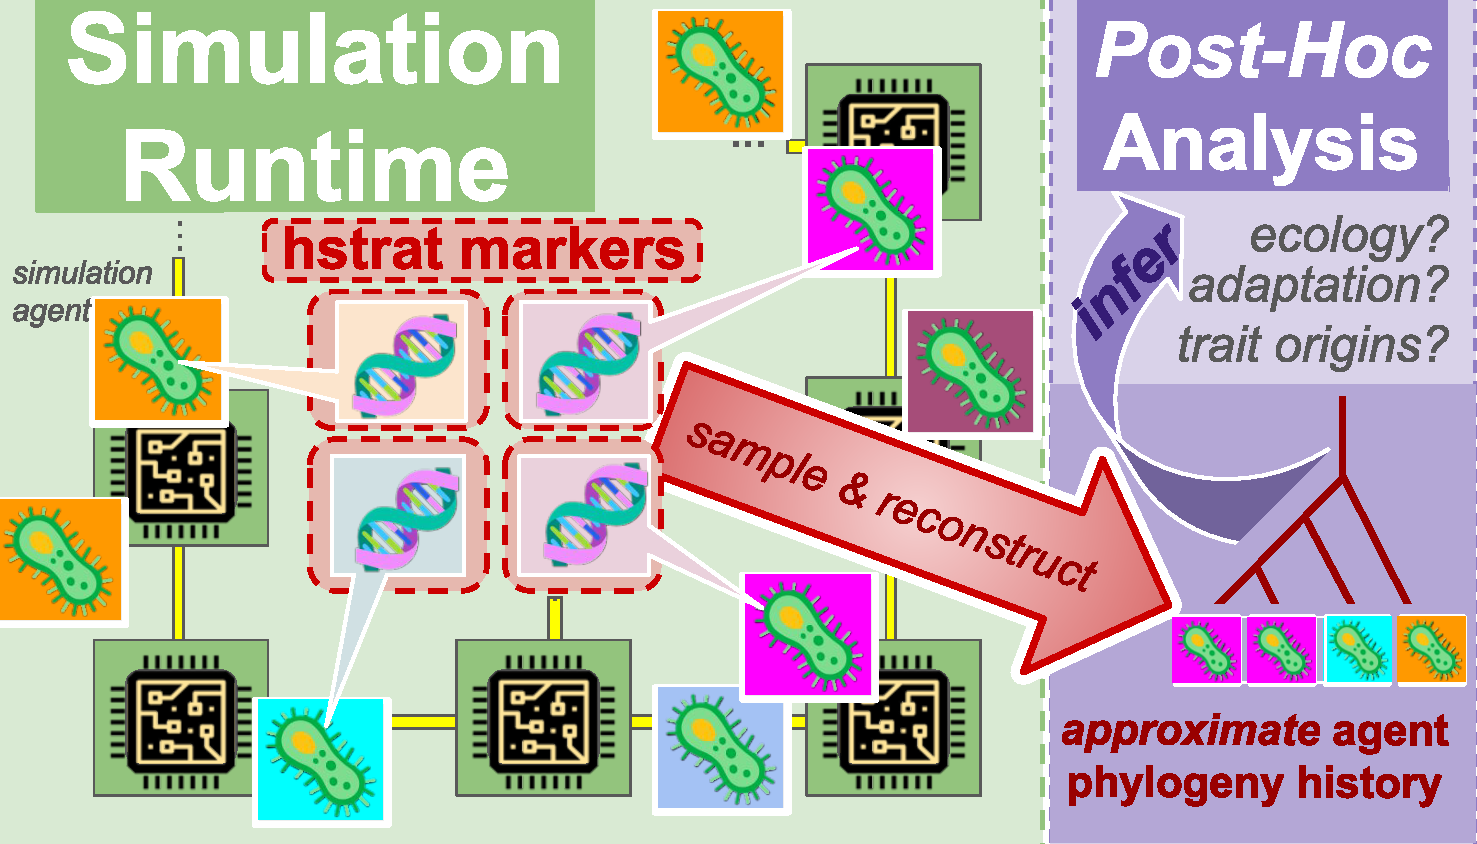
\includegraphics[width=2in]{img/runtime-posthoc-schematic.pdf}
% \end{minipage}%
% \begin{minipage}{2in}
\vspace{-5ex}
\caption{\footnotesize
Evolution simulation with reconstruction-based lineage analysis.}
\label{fig:runtime-posthoc-schematic}
\vspace{-2ex}
% \end{minipage}
\end{wrapfigure}


In recent work, we have taken major strides towards this vision with the Cerebras SDK, phylogenetic reconstruction using hereditary stratigraphy techniques and managing a population using asynchronous agent migration between neighboring PEs.

\section{Science Question}
What is the structural relationship between individual-level phylogenies and species-level phylogenies? Do they respond in the same way to evolutionary conditions like selection pressure, ecology, and spatial structure?

What conditions precipitate emergence/success of new viral strains? In particular, how does the population size/infection intensity affect the rate at which strains emerge/sweep?  [get citation from marisa?]

\section{Engineering Questions}
Possible topics appropriately scoped engineering questions behind this science question for the workshop environment include,
\begin{itemize}
\item How to efficiently perform long-distance migration?
One possibility is to impose an overlay of fixed long distance routes.
Another would be stochastic forwarding.
How best to take advantage of built-routing capabilities will benefit from instruction in the workshop.
This is important to be able to create more realistic population structures that deviate beyond simple grid connectivity.
\item How to sample population members on-the-fly?
The builtin memcpy operation provides a good way to do this at conclusion, but advanced techniques for asynchronous memcpy operations or otherwise.
\end{itemize}

https://github.com/mmore500/wse-sketches

\section{Broader Impacts}

The availability of modular, extendable software for agent-based evolution simulation on emerging HPC architectures will catalyze research. Progress on this front
How to organize and distribute CSL modules.
If there aren’t established protocols, the workshop environment would be a great place to discuss these issues.

ADD PERSONAL STATEMENT CONTENT HERE

This work lays foundations for research in open—ended evolution (cite MODES) and in evolutionary epidemiology, among other topics. (move to intro?)
